\documentclass[spanish,letterpaper,oneside]{article}

\def\documenttitle {Historia y origen del Estado}
\def\documentsubtitle {Formaciones politicas y limites del poder}
\def\documentsubject {Actividad 2 - Teoria del Estado y Constitucion}
\def\documentauthor {Martin Jonathan de la Cruz}
\def\coursename {Teoria del Estado y Constitucion}
\def\coursecode {020}
\def\universityname {Universidad Abierta y a Distancia de Mexico}
\def\universityfaculty {Licenciatura en Derecho}
\def\universitydepartment {Teoria del Estado y Constitucion}
\def\universitydepartmentimage {departamentos/UnADM}
\def\universitydepartmentimagecfg {height=1.57cm}
\def\universitylocation {Roma Norte, Ciudad de Mexico}
\def\authortable {
  \begin{tabular}{ll}
    \textbf{Alumno:} & Martin Jonathan de la Cruz \\
    Matricula: & ES2611202040 \\
    Figura docente: & Ana Lilian Sanchez Chavez \\
    Semestre/Bloque: & 2 / 2 \\
    Semana: & 2 \\
    \multicolumn{2}{l}{Fecha de realizacion: \today} \\
    \multicolumn{2}{l}{\universitylocation}
  \end{tabular}
}

\input{template}
\usepackage{helvet}
\renewcommand{\familydefault}{\sfdefault}
\usepackage{array}
\usepackage{booktabs}
\usepackage{longtable}
\usepackage{calc}
\usepackage{tikz}
\usepackage{pdflscape}
\usetikzlibrary{arrows.meta,positioning,calc,babel}
\setcitestyle{authoryear,open={(},close={)}}
\providecommand{\tightlist}{\setlength{\itemsep}{0pt}\setlength{\parskip}{0pt}}
\providecommand{\pandocbounded}[1]{#1}
\providecommand{\passthrough}[1]{#1}
\setlength{\emergencystretch}{3em}

\def\coverwatermarkenabled {true}
\def\coverwatermarkimage {img/departamentos/UnADM.pdf}
\def\coverwatermarkopacity {0.16}
\def\coverwatermarkwidth {0.72\paperwidth}
\def\coverwatermarkxshift {0cm}
\def\coverwatermarkyshift {-0.35cm}
\newcommand{\insertcoverwatermark}{%
  \ifthenelse{\equal{\coverwatermarkenabled}{true}}{%
    \AddToShipoutPictureBG*{%
      \begin{tikzpicture}[remember picture,overlay]
        \node[opacity=\coverwatermarkopacity,inner sep=0pt,
          xshift=\coverwatermarkxshift,yshift=\coverwatermarkyshift]
          at (current page.center) {%
            \includegraphics[width=\coverwatermarkwidth]{\coverwatermarkimage}%
          };
      \end{tikzpicture}%
    }%
  }{}%
}

\begin{document}
\insertcoverwatermark
\templatePortrait
\templatePagecfg
\onehalfspacing
\templateIndex
\templateFinalcfg

\section{Introduccion}

El origen del Estado no puede explicarse como una sucesion inevitable de
formas politicas cada vez mejores. La administracion de recursos, la
concentracion de autoridad y los limites juridicos del poder responden a
problemas distintos. Uruk ofrece un antecedente urbano de gestion de
bienes; la Carta Magna muestra un limite pactado frente al monarca;
Versalles representa la centralizacion absolutista; la Declaracion de
1789 vincula soberania y derechos, mientras el constitucionalismo exige
instituciones capaces de hacer efectivos esos limites
\citep{metUruk2003,parliamentMagnaCarta,versaillesLouisXIV,francia1789,garciaRicci2011}.

La comparacion se concentra en antecedentes mesopotamicos, europeos y
su proyeccion juridica mexicana, sin convertir esa seleccion en una
historia universal. Las cinco etapas son referencias de lectura:
el Estado moderno se forma durante la temprana modernidad y, por ello,
se superpone al absolutismo; no nace exclusivamente despues de 1789.
La distincion entre organizacion estatal y Estado de derecho permite
examinar tanto la capacidad de gobernar como la legitimidad de sus fines
\citep{garciaRicci2011}.

\clearpage
\section{Formaciones politicas y limites del poder}
\subsection{Antecedentes y criterios de comparacion}

La gestion de bienes y raciones documentada en Uruk hacia 3200 a.~C.
permite relacionar organizacion economica con administracion urbana,
sin identificar esa ciudad con una nacion contemporanea
\citep{metUruk2003}. En 1215, una crisis politica y la presion de los
barones ingleses dieron lugar a un instrumento que limito la autoridad
real; no fue concebido como una carta de derechos para todas las
personas \citep{parliamentMagnaCarta}.

En Francia, la reorganizacion administrativa y financiera y el traslado
de la corte a Versalles en 1682 reforzaron un poder centrado en el
monarca \citep{versaillesLouisXIV}. La razon de Estado plantea aqui una
tension analitica: conservar capacidad de gobierno no equivale a
justificar cualquier medio utilizado para conservarla.

La Declaracion de 1789 ofrece otro criterio de legitimacion: igualdad
juridica (art.~1), soberania nacional (art.~3), ley como expresion de la
voluntad general (art.~6) y garantia de derechos y separacion de poderes
(art.~16) \citep{francia1789}. En Mexico, los articulos 1, 39--41 y 49
constitucionales permiten contrastar proteccion de derechos, soberania
popular, forma de gobierno y division del poder
\citep{cpeum2026S2}.

\subsection{Historia y origen del Estado}
La figura~\ref{fig:linea-estado} relaciona una fecha representativa con
un acontecimiento, su causa o consecuencia y una valoracion critica en
cada etapa. El orden indica sucesion de hitos, no duraciones a escala.
Las etapas se superponen y sus limites no son universales; 1917 funciona
como hito mexicano de constitucionalismo, no como fecha de nacimiento
del Estado moderno.
Los ocho hitos conservan las cinco etapas requeridas y distinguen
formacion moderna, constitucionalismo e internacionalizacion de los
derechos. Versalles ilustra la centralizacion, no todo el periodo;
la portada de 1917 se reutiliza en 2011 como simbolo constitucional,
no como reproduccion del decreto de reforma.

\begin{landscape}
\thispagestyle{empty}
\begingroup
\setstretch{1.05}
\begin{images}[\label{fig:linea-estado}]{Historia y origen del Estado: ocho hitos, distancias no proporcionales. Imagenes: Warka, O. S. Muhammed Amin (CC BY-SA 4.0); Versalles, ToucanWings (CC BY-SA 3.0); Eleanor Roosevelt, FDR Presidential Library \& Museum (CC BY 2.0); documentos, dominio publico. Wikimedia Commons.}
\resizebox{\linewidth}{!}{%
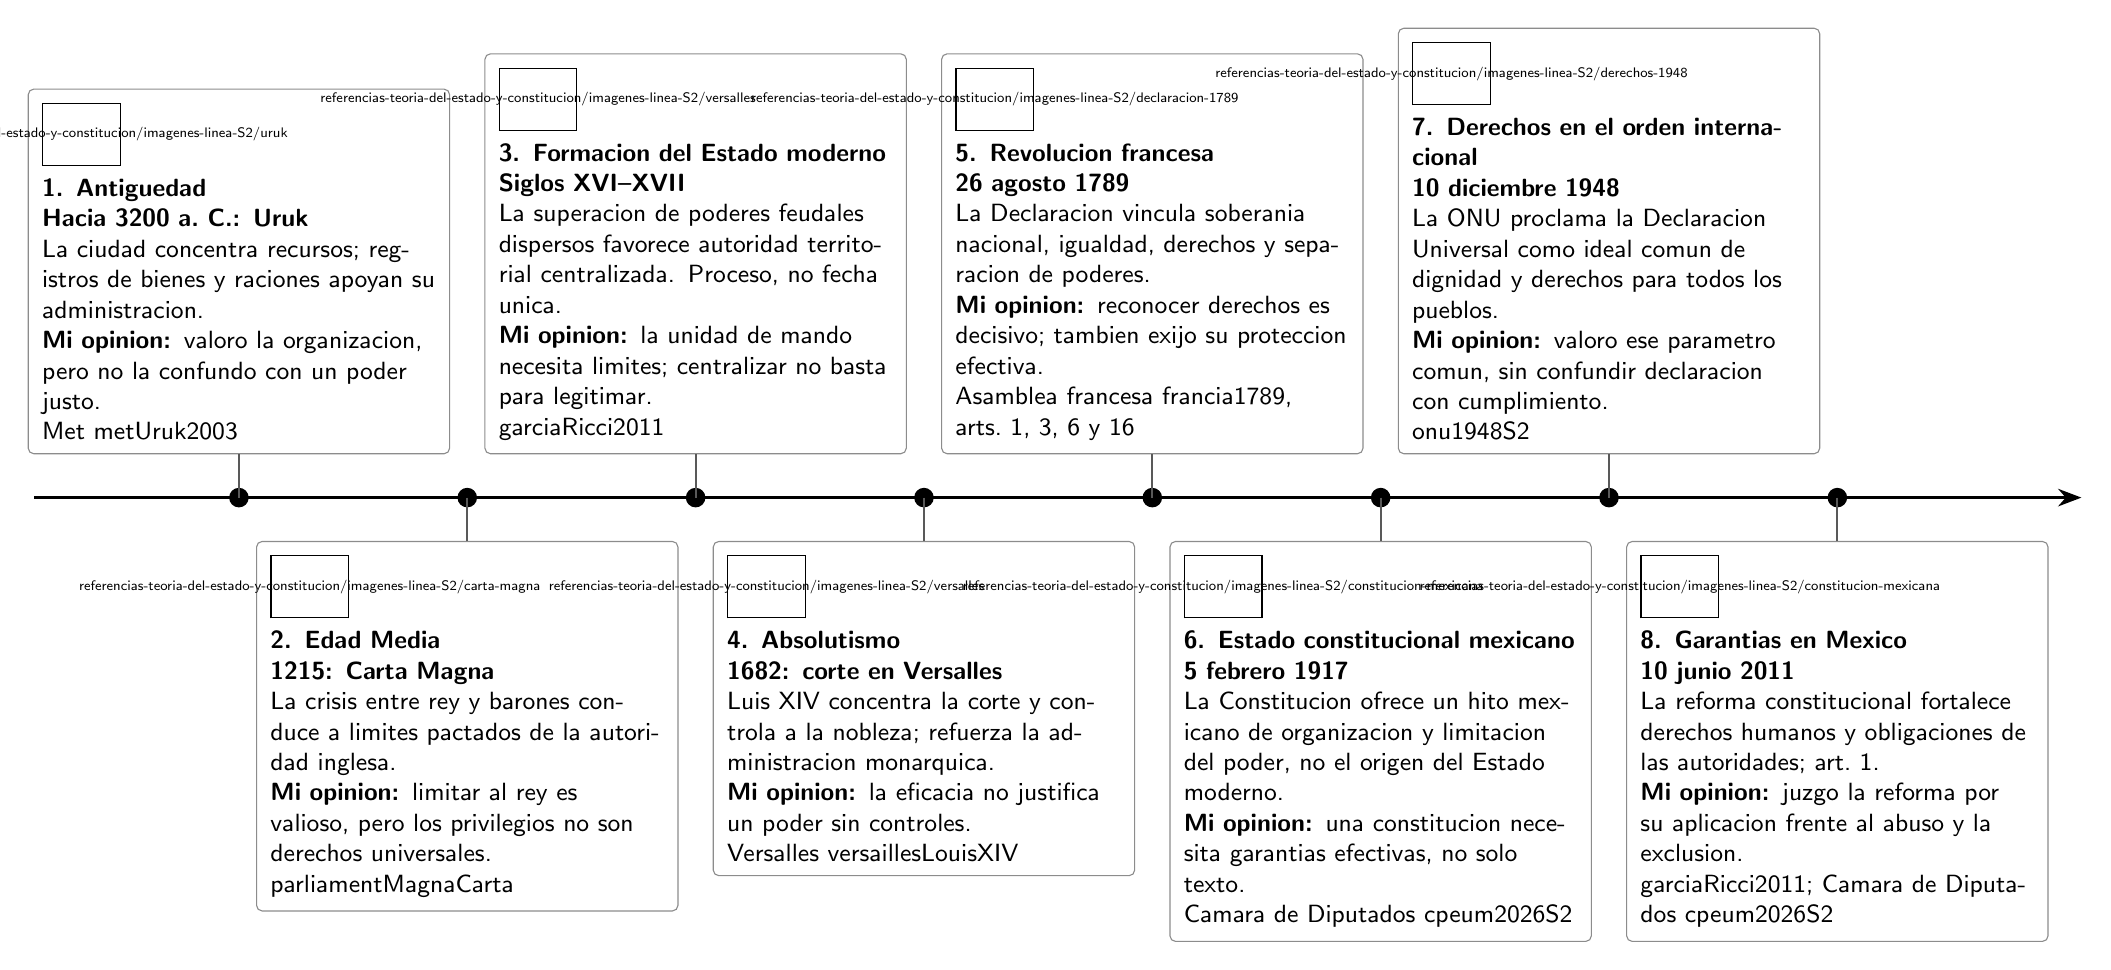
\begin{tikzpicture}[
  panel/.style={draw=black!45,fill=white,rounded corners=2pt,
    text width=5cm,align=left,inner sep=5pt,font=\small},
  enlace/.style={draw=black!65,line width=0.8pt},
  hito/.style={circle,fill=black,inner sep=2.5pt}]
\draw[-{Stealth},line width=1.2pt] (0,0) -- (26,0);
\node[panel,anchor=south] (antigua) at (2.6,0.55) {
  \pgfimage[height=0.8cm]{referencias-teoria-del-estado-y-constitucion/imagenes-linea-S2/uruk}\par
  \textbf{1. Antiguedad}\par
  \textbf{Hacia 3200 a.~C.: Uruk}\par
  La ciudad concentra recursos; registros de bienes y raciones apoyan su administracion.\par
  \textbf{Mi opinion:} valoro la organizacion, pero no la confundo con un poder justo.\par
  Met \citeyearpar{metUruk2003}};
\node[panel,anchor=north] (medieval) at (5.5,-0.55) {
  \pgfimage[height=0.8cm]{referencias-teoria-del-estado-y-constitucion/imagenes-linea-S2/carta-magna}\par
  \textbf{2. Edad Media}\par
  \textbf{1215: Carta Magna}\par
  La crisis entre rey y barones conduce a limites pactados de la autoridad inglesa.\par
  \textbf{Mi opinion:} limitar al rey es valioso, pero los privilegios no son derechos universales.\par
  \citep{parliamentMagnaCarta}};
\node[panel,anchor=south] (formacion) at (8.4,0.55) {
  \pgfimage[height=0.8cm]{referencias-teoria-del-estado-y-constitucion/imagenes-linea-S2/versalles}\par
  \textbf{3. Formacion del Estado moderno}\par
  \textbf{Siglos XVI--XVII}\par
  La superacion de poderes feudales dispersos favorece autoridad territorial centralizada. Proceso, no fecha unica.\par
  \textbf{Mi opinion:} la unidad de mando necesita limites; centralizar no basta para legitimar.\par
  \citep{garciaRicci2011}};
\node[panel,anchor=north] (absoluto) at (11.3,-0.55) {
  \pgfimage[height=0.8cm]{referencias-teoria-del-estado-y-constitucion/imagenes-linea-S2/versalles}\par
  \textbf{4. Absolutismo}\par
  \textbf{1682: corte en Versalles}\par
  Luis XIV concentra la corte y controla a la nobleza; refuerza la administracion monarquica.\par
  \textbf{Mi opinion:} la eficacia no justifica un poder sin controles.\par
  Versalles \citeyearpar{versaillesLouisXIV}};
\node[panel,anchor=south] (francesa) at (14.2,0.55) {
  \pgfimage[height=0.8cm]{referencias-teoria-del-estado-y-constitucion/imagenes-linea-S2/declaracion-1789}\par
  \textbf{5. Revolucion francesa}\par
  \textbf{26 agosto 1789}\par
  La Declaracion vincula soberania nacional, igualdad, derechos y separacion de poderes.\par
  \textbf{Mi opinion:} reconocer derechos es decisivo; tambien exijo su proteccion efectiva.\par
  Asamblea francesa \citeyearpar{francia1789}, arts.~1, 3, 6 y 16};
\node[panel,anchor=north] (moderno) at (17.1,-0.55) {
  \pgfimage[height=0.8cm]{referencias-teoria-del-estado-y-constitucion/imagenes-linea-S2/constitucion-mexicana}\par
  \textbf{6. Estado constitucional mexicano}\par
  \textbf{5 febrero 1917}\par
  La Constitucion ofrece un hito mexicano de organizacion y limitacion del poder, no el origen del Estado moderno.\par
  \textbf{Mi opinion:} una constitucion necesita garantias efectivas, no solo texto.\par
  Camara de Diputados \citeyearpar{cpeum2026S2}};
\node[panel,anchor=south] (universal) at (20,0.55) {
  \pgfimage[height=0.8cm]{referencias-teoria-del-estado-y-constitucion/imagenes-linea-S2/derechos-1948}\par
  \textbf{7. Derechos en el orden internacional}\par
  \textbf{10 diciembre 1948}\par
  La ONU proclama la Declaracion Universal como ideal comun de dignidad y derechos para todos los pueblos.\par
  \textbf{Mi opinion:} valoro ese parametro comun, sin confundir declaracion con cumplimiento.\par
  \citep{onu1948S2}};
\node[panel,anchor=north] (reforma) at (22.9,-0.55) {
  \pgfimage[height=0.8cm]{referencias-teoria-del-estado-y-constitucion/imagenes-linea-S2/constitucion-mexicana}\par
  \textbf{8. Garantias en Mexico}\par
  \textbf{10 junio 2011}\par
  La reforma constitucional fortalece derechos humanos y obligaciones de las autoridades; art.~1.\par
  \textbf{Mi opinion:} juzgo la reforma por su aplicacion frente al abuso y la exclusion.\par
  \citep{garciaRicci2011}; Camara de Diputados \citeyearpar{cpeum2026S2}};
\foreach \pos/\lado in {2.6/0.55,5.5/-0.55,8.4/0.55,11.3/-0.55,14.2/0.55,17.1/-0.55,20/0.55,22.9/-0.55} {
  \node[hito] at (\pos,0) {};
  \draw[enlace] (\pos,0) -- (\pos,\lado);
}
\end{tikzpicture}
}
\end{images}
\endgroup
\end{landscape}

\subsection{Continuidades, rupturas y consecuencias}

La Declaracion Universal de 1948 introduce un parametro comun de
dignidad y derechos para todos los pueblos. No es un tratado ni acredita
por si sola cumplimiento efectivo. En Mexico, la reforma del 10 de junio
de 2011 fortalece el marco constitucional de derechos humanos y las
obligaciones de promover, respetar, proteger y garantizar esos derechos.
Ambos hitos amplian el criterio de evaluacion del poder mas alla de su
capacidad de administrar \citep{onu1948S2,garciaRicci2011,cpeum2026S2}.

La continuidad principal es la necesidad de organizar recursos y
autoridad; cambia la forma de justificar y limitar esa autoridad.
Los registros de Uruk permiten observar administracion, pero no deben
leerse como evidencia de ciudadania moderna. La Carta Magna limita
determinadas actuaciones reales mediante un acuerdo desigual en sus
beneficiarios. Ambos ejemplos muestran por que conviene distinguir
existencia de reglas, distribucion del poder y alcance de la proteccion
\citep{metUruk2003,parliamentMagnaCarta}.

Versalles muestra que centralizar puede fortalecer la capacidad de
gobierno sin repartir de manera igual el poder. La Declaracion de 1789
desplaza el criterio normativo hacia soberania y derechos: su articulo
12 exige una fuerza publica para beneficio de todos, no de quienes la
ejercen. Esa exigencia cuestiona la identificacion entre interes del
gobernante e interes colectivo \citep{versaillesLouisXIV,francia1789}.

En Mexico, el articulo 39 hace derivar el poder publico del pueblo y
lo instituye para su beneficio; el articulo 49 distribuye el Supremo
Poder de la Federacion. Para el ejercicio juridico, esa relacion permite
examinar una decision publica preguntando por su competencia, su
fundamento y sus mecanismos de control, en vez de aceptar su legitimidad
solo por provenir de una autoridad \citep{cpeum2026S2,garciaRicci2011}.

\clearpage
\section{Conclusiones}

La historia del Estado permite separar tres dimensiones: organizacion
de recursos, concentracion de autoridad y legitimacion juridica.
Uruk, Carta Magna, Versalles y la Declaracion de 1789 ilustran respuestas
distintas a esas cuestiones; no forman una escala automatica de progreso.
El constitucionalismo incorpora una exigencia adicional: la autoridad
debe sujetarse a limites y proteger derechos, no solo administrar con
eficacia \citep{garciaRicci2011,francia1789}.

Considero que el fin del Estado no debe confundirse con la permanencia
de sus gobernantes. Reconozco la importancia de administrar recursos y
mantener instituciones estables, pero entiendo que esa capacidad pierde
legitimidad cuando deja de servir a las personas. Mi razon es juridica:
si el poder se instituye en beneficio del pueblo, debe ejercerse dentro
de competencias y someterse a controles que protejan sus derechos
\citep[arts.~1, 39 y 49]{cpeum2026S2}.

Desde mi formacion en Derecho, encuentro en esta comparacion un criterio
para evaluar decisiones publicas: preguntar quien tiene competencia,
con que fundamento actua y que medios existen para cuestionar un abuso.
No considero suficiente que una autoridad invoque orden o estabilidad;
me interesa que sus decisiones puedan justificarse y revisarse.
Por eso valoro el constitucionalismo como una exigencia de limites
efectivos, no como una garantia automatica de justicia.
Al interpretar estos procesos, distingo los hechos documentados de mi
valoracion critica.\footnote{Se utilizo GitHub Copilot para apoyar
la organizacion de fuentes, la redaccion y la construccion del diagrama.
La asistencia no sustituye el analisis propio ni la revision personal
de los argumentos y de las fuentes antes de entregar.}

\clearpage
\begin{thebibliography}{7}
\bibitem[Asamblea Nacional Constituyente de Francia(1789)]{francia1789}
Asamblea Nacional Constituyente de Francia. (1789, 26 de agosto).
\emph{Declaration of Human and Civic Rights of 26 August 1789}.
Conseil constitutionnel.
\url{https://www.conseil-constitutionnel.fr/en/declaration-of-human-and-civic-rights-of-26-august-1789}

\bibitem[Camara de Diputados del H. Congreso de la Union(2026)]{cpeum2026S2}
Camara de Diputados del H. Congreso de la Union. (2026).
\emph{Constitucion Politica de los Estados Unidos Mexicanos}
(ultima reforma publicada en el DOF el 7 de octubre de 2026).
\url{https://www.diputados.gob.mx/LeyesBiblio/pdf/CPEUM.pdf}

\bibitem[Department of Ancient Near Eastern Art(2003)]{metUruk2003}
Department of Ancient Near Eastern Art. (2003, octubre).
\emph{Uruk: The first city}. The Metropolitan Museum of Art.
\url{https://www.metmuseum.org/essays/uruk-the-first-city}

\bibitem[Garcia Ricci(2011)]{garciaRicci2011}
Garcia Ricci, D. (2011). \emph{Estado de derecho y principio de legalidad}.
Comision Nacional de los Derechos Humanos.
\url{https://corteidh.or.cr/tablas/r28801.pdf}

\bibitem[Naciones Unidas(1948)]{onu1948S2}
Naciones Unidas. (1948, 10 de diciembre).
\emph{Declaracion Universal de Derechos Humanos}.
\url{https://www.un.org/en/about-us/universal-declaration-of-human-rights}

\bibitem[Palace of Versailles(s.\,f.)]{versaillesLouisXIV}
Palace of Versailles. (s.\,f.). \emph{Louis XIV}.
\url{https://en.chateauversailles.fr/discover/history/great-characters/louis-xiv}

\bibitem[UK Parliament(s.\,f.)]{parliamentMagnaCarta}
UK Parliament. (s.\,f.). \emph{Magna Carta}.
\url{https://www.parliament.uk/about/living-heritage/evolutionofparliament/originsofparliament/birthofparliament/overview/magnacarta/}
\end{thebibliography}

\end{document}